\section[Morphological Metrics]{Morphological Analysis of Airway Trees}
\label{sec:morphometrics}                % \secref{sec:morphometrics} -- used by the Labelling section
\label{sec:morph}                        % same place, name used in the draft

Once every airway tree is anatomically labeled (\secref{sec:labeling}), we describe its shape
with the six morphological descriptors of AirwaySignature, introduced with the AirMorph
framework by \citet{zhang2025airmorph}: Stenosis ($S$), Ectasia ($E$), Tortuosity ($T$),
Length ($L$), Divergence ($D$) and Complexity ($C$). The descriptors capture local variations
in airway shape that cannot be seen from the binary segmentation alone and they are defined
per anatomical class, so that each value refers to a specific bronchus (a segmental or a
lobar branch) \cite{zhang2025airmorph}. For each tree, the result is a compact, anatomically
aligned signature, one value of each descriptor for every anatomical class present in the
tree Figure~\ref{fig:morph_ours}..

% ------------------------------------------------------------------------------
\subsection{Overview}                    % the two groups of descriptors
\label{sec:morph_overview}               % \secref{sec:morph_overview}

\citet{zhang2025airmorph} divide the six descriptors into two groups
(Figure~\ref{fig:morph_def}):
\begin{itemize}                          % the two descriptor groups
  \item \textbf{Branch-level descriptors} ($S$, $E$, $T$) are first computed on each
        individual branch of the airway skeleton and then averaged over all branches that
        belong to the same anatomical class. Stenosis measures the strongest narrowing
        of a branch, Ectasia its strongest dilation, and Tortuosity how much its 3D
        trajectory bends.
  \item \textbf{Subtree-level descriptors} ($L$, $D$, $C$) are computed on the whole
        subtree of an anatomical class, i.e.\ on all connected branches that share the same
        anatomical context. Length measures the geodesic length of the subtree,
        Divergence the angular spread of its terminal branches, and Complexity the
        irregularity and density of its branching through a fractal dimension.
\end{itemize}
The anatomical class $K$ over which the descriptors are grouped can be a segmental or a
lobar bronchus \cite{zhang2025airmorph}. In our case the labels come from IPGN, which
provides 18 segmental classes. The lobar classes were obtained by merging the segmental
labels of each lobe / we computed the descriptors at segmental level only.

Table~\ref{tab:morph_summary} summarizes the six descriptors.

\begin{table}[htbp]                      % summary of the six descriptors
  \centering                             % center the table
  \small                                 % slightly smaller font so the table fits
  \caption{The six AirwaySignature descriptors of \citet{zhang2025airmorph}.}
  \label{tab:morph_summary}              % referenced as Table~\ref{tab:morph_summary}
  \begin{tabular}{llll}                  % name, level, range, higher value means
    \toprule
    Descriptor & Computed on & Range & Higher value means \\
    \midrule
    Stenosis ($S$)    & Each branch, then averaged & $[0\%, 100\%]$ & stronger narrowing \\
    Ectasia ($E$)     & Each branch, then averaged & $[100\%, +\infty)$ & stronger dilation \\
    Tortuosity ($T$)  & Each branch, then averaged & $[0, 1]$ & stronger bending \\
    Length ($L$)      & Class subtree & $[0, +\infty)$ mm & longer subtree \\
    Divergence ($D$)  & Class subtree & $[0, 1]$ & wider angular spread \\
    Complexity ($C$)  & Class subtree & $[0, +\infty)$ & more complex branching \\
    \bottomrule
  \end{tabular}
\end{table}

\begin{figure}[htbp]                     % placeholder for the descriptor definition figure
  \centering                             % center the figure
  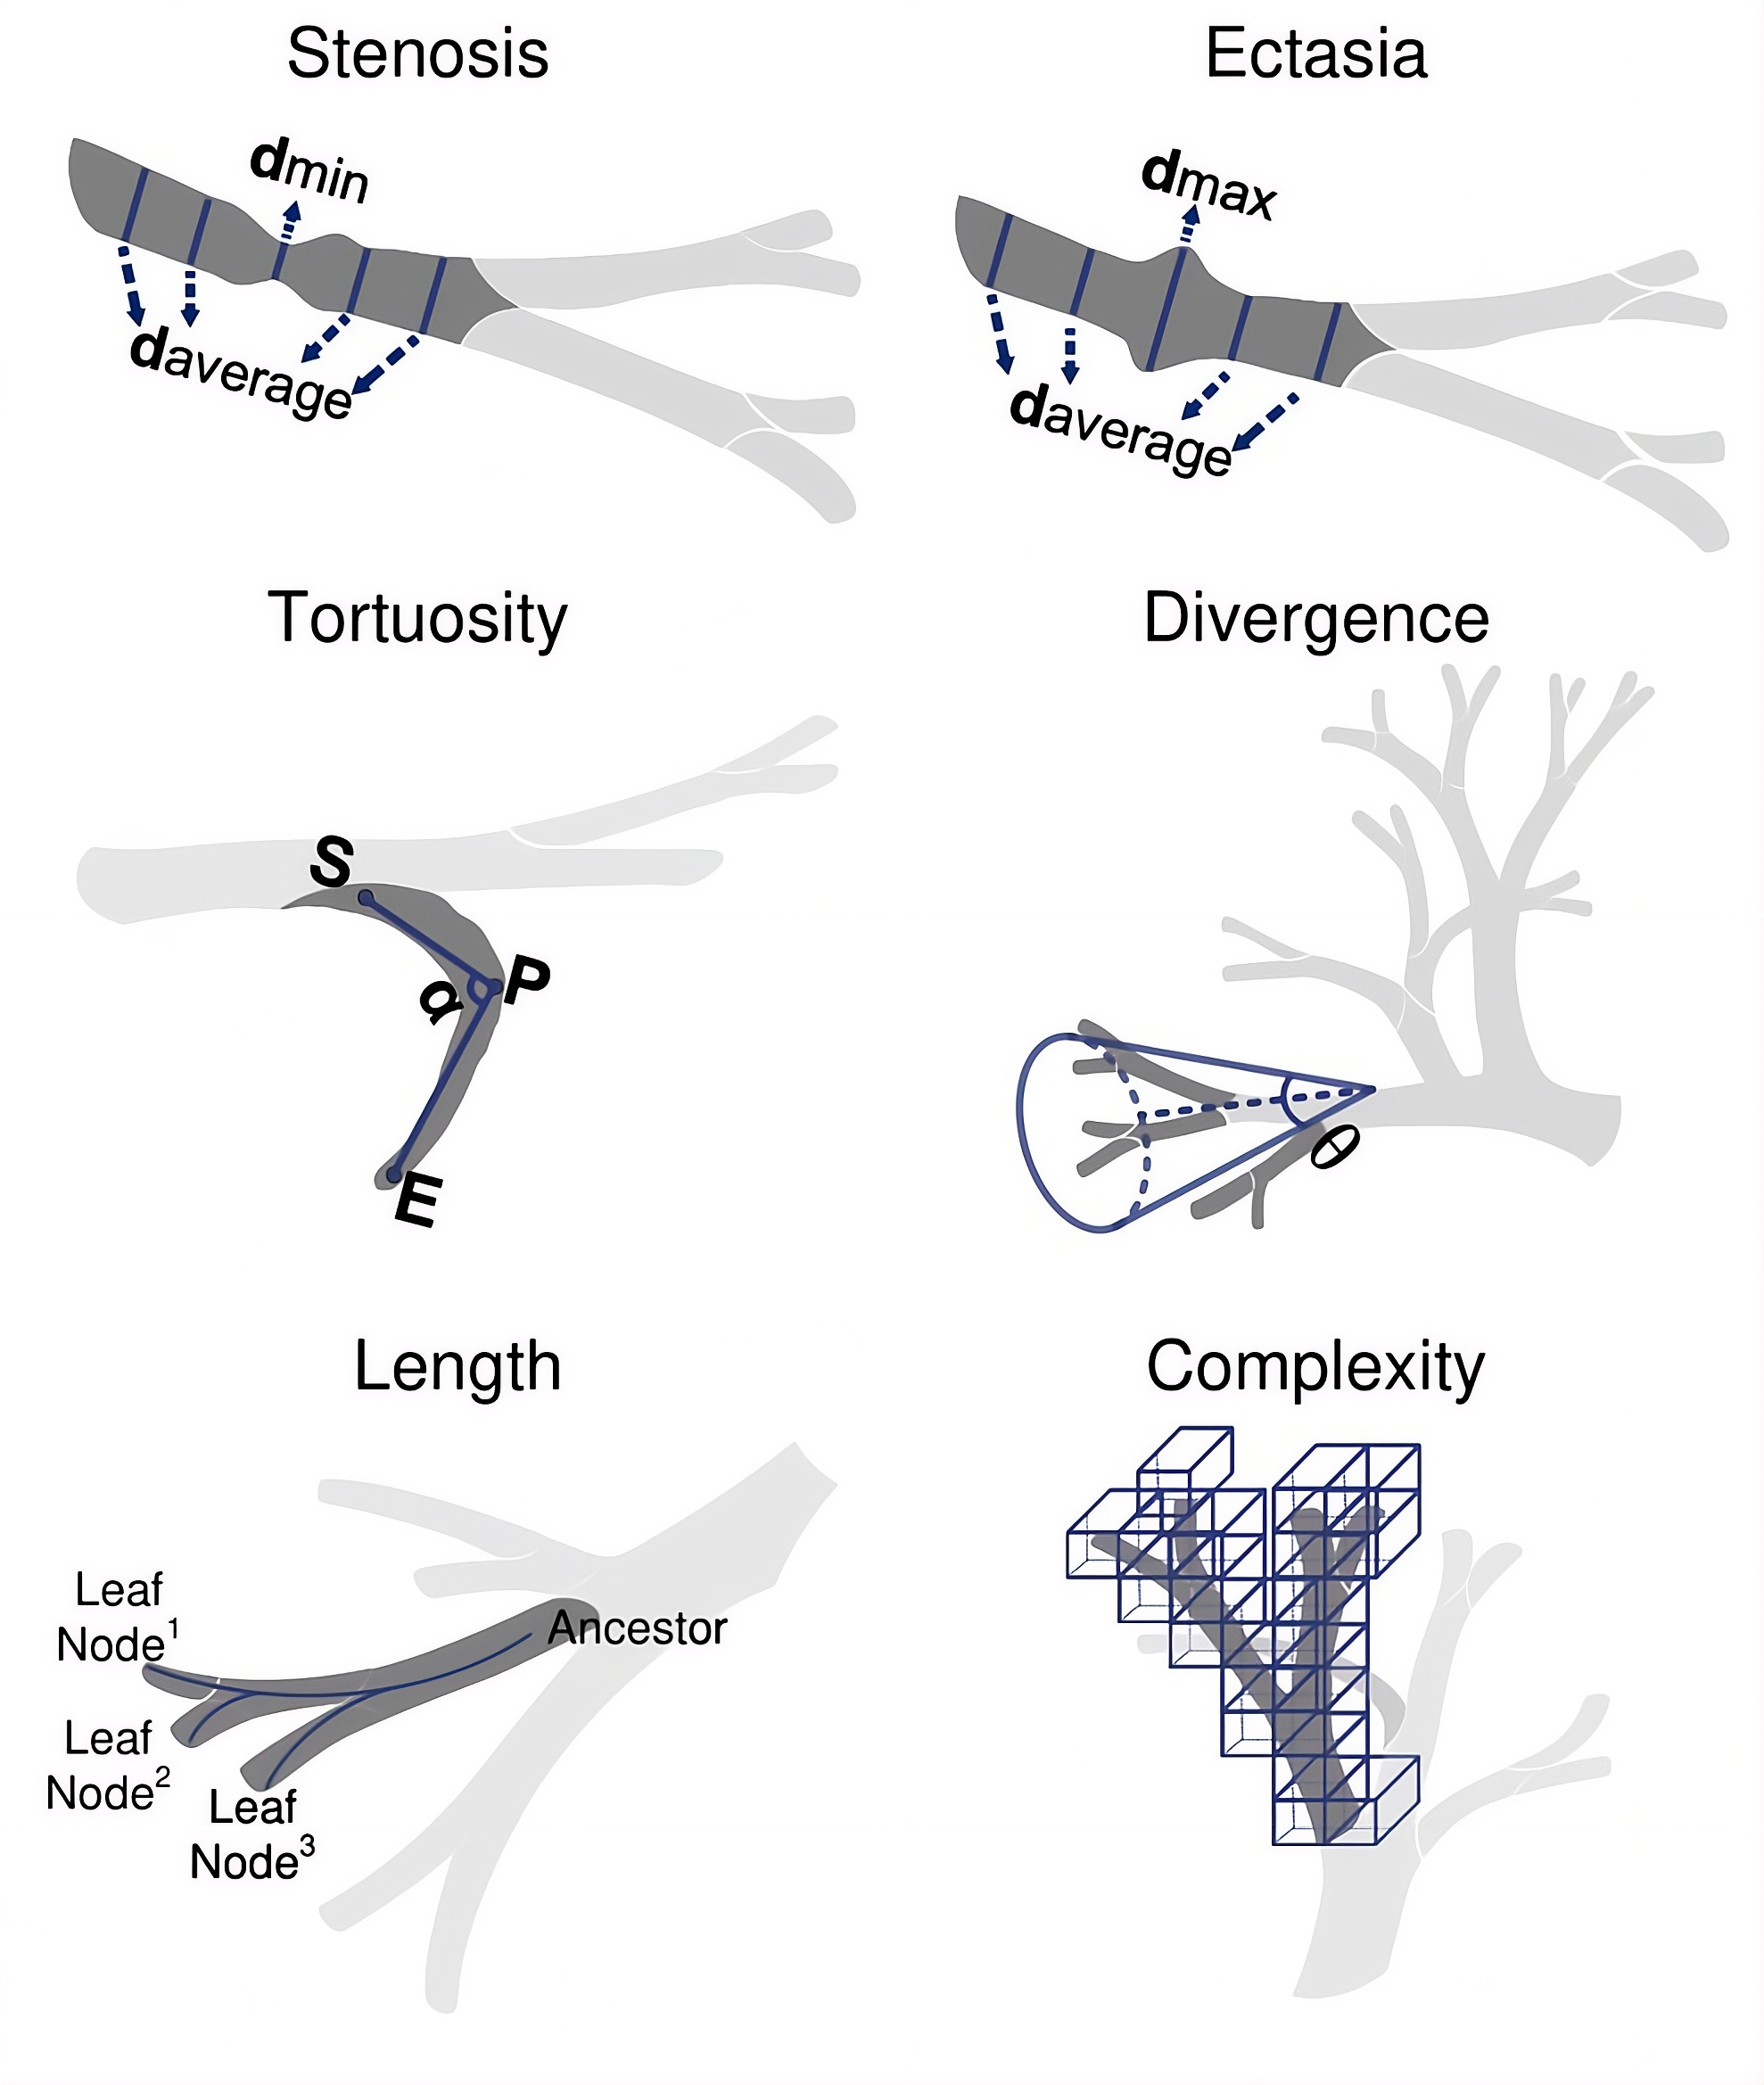
\includegraphics[width=\textwidth]{figures/morphological_metrics.png}  % uncomment with your file
  \caption{The six morphological descriptors of AirwaySignature from
           \citet{zhang2025airmorph}.}
  \label{fig:morph_def}                  % referenced as Figure~\ref{fig:morph_def}
\end{figure}

% ------------------------------------------------------------------------------
\subsection{Common pre-processing}       % radius field and skeleton parsing
\label{sec:morph_preproc}                % \secref{sec:morph_preproc}

Stenosis and Ectasia are both based on the local airway radius along the centerline, which is
obtained as follows \cite{zhang2025airmorph}:
\begin{enumerate}                        % the radius-extraction steps
  \item \textbf{Radius field.} A 3D Euclidean distance transform (EDT) is applied to the
        binary airway mask $V_{\mathrm{airway}}$, taking the voxel spacing $s$ into
        account. At every foreground voxel it gives the distance to the nearest background
        voxel, i.e.\ an approximation of the local airway radius in mm.
  \item \textbf{Centerline radii.} The distance field is masked with the airway skeleton
        $\mathcal{S}$, keeping only the values on centerline voxels. This gives the
        radius field along the skeleton:
        \begin{equation}
          R = \mathrm{EDT}(V_{\mathrm{airway}}; s) \cdot \mathcal{S}.
          \label{eq:morph_radius}        % radius restricted to the skeleton
        \end{equation}
  \item \textbf{Skeleton parsing.} The skeleton is split into individual branches using a
        26-connected neighborhood and removing the junction voxels, so that each branch is
        spatially isolated. Each parsed branch $b$ receives the anatomical label of the
        region it lies in.
\end{enumerate}
For every parsed branch $b$, the minimum, mean and maximum radius along its centerline are
then computed:
\begin{equation}
  r^{(b)}_{\min} = \min_{x \in b} R(x), \qquad
  r^{(b)}_{\mathrm{mean}} = \frac{1}{|b|} \sum_{x \in b} R(x), \qquad
  r^{(b)}_{\max} = \max_{x \in b} R(x).
  \label{eq:morph_rstats}                % per-branch radius statistics
\end{equation}

% ------------------------------------------------------------------------------
\subsection{Branch-level descriptors}    % stenosis, ectasia, tortuosity
\label{sec:morph_branch}                 % \secref{sec:morph_branch}

\paragraph{Stenosis ($S$).}              % narrowing
Stenosis quantifies airway narrowing. \citet{zhang2025airmorph} define it as the reduction of
the radius at the point of strongest constriction, $R_{\mathrm{narrow}}$, relative to a
reference radius $R_{\mathrm{ref}}$, the mean radius of a healthy proximal airway segment:
\begin{equation}
  \mathrm{Stenosis} = \left(1 - \frac{R_{\mathrm{narrow}}}{R_{\mathrm{ref}}}\right)
  \times 100\%.
  \label{eq:morph_stenosis_def}          % conceptual stenosis definition
\end{equation}
In their implementation, both quantities are taken from the radius statistics of each
parsed branch: $R_{\mathrm{narrow}}$ is the branch's minimum radius and $R_{\mathrm{ref}}$
its mean radius, which gives the local stenosis ratio of branch $b$:
\begin{equation}
  S_b = 1 - \frac{r^{(b)}_{\min}}{r^{(b)}_{\mathrm{mean}}}.
  \label{eq:morph_stenosis_branch}       % per-branch stenosis as implemented
\end{equation}
The stenosis of an anatomical class $K$ is the average over all branches carrying that label:
\begin{equation}
  S_K = \frac{1}{|B_K|} \sum_{b \in B_K} S_b,
  \label{eq:morph_stenosis_class}        % class-level stenosis
\end{equation}
where $B_K$ is the set of parsed branches with label $K$. If a class is absent from the tree,
its score is set to $-1$ \cite{zhang2025airmorph}. Stenosis ranges from 0\% to 100\%, and
higher values mean a more severe narrowing.

\paragraph{Ectasia ($E$).}               % dilation
Ectasia complements Stenosis: instead of narrowing, it captures over-expansion of the airway
lumen \cite{zhang2025airmorph}. It is defined as the ratio between the maximum radius and the
reference radius, which in the implementation is again the mean radius of each parsed branch:
\begin{equation}
  \mathrm{Ectasia} = \frac{R_{\max}}{R_{\mathrm{ref}}} \times 100\%,
  \qquad
  E_b = \frac{r^{(b)}_{\max}}{r^{(b)}_{\mathrm{mean}}}.
  \label{eq:morph_ectasia}               % per-branch ectasia
\end{equation}
As for Stenosis, the class value $E_K$ is the average of $E_b$ over all branches with label
$K$, and absent classes receive $-1$. Ectasia ranges from 100\% upwards, and higher values
mean a stronger dilation \cite{zhang2025airmorph}.

\paragraph{Tortuosity ($T$).}            % bending of a branch
Tortuosity describes the local curvature of a branch from its volumetric
geometry \cite{zhang2025airmorph}. For a branch region $\Omega_l$ (the set of its voxels):
\begin{enumerate}                        % the tortuosity steps
  \item the voxel coordinates are converted to physical space using the voxel spacing;
  \item principal component analysis (PCA) is applied to these coordinates, and the two
        endpoints $\mathbf{S}$ and $\mathbf{E}$ of the branch are taken along the first
        principal axis, i.e.\ the main direction of the branch;
  \item the voxel $\mathbf{P}$ that lies furthest from the segment $\overline{SE}$ is
        found:
        \begin{equation}
          \mathbf{P} = \arg\max_{\mathbf{x}_i \in \Omega_l}
              \mathrm{dist}\big(\mathbf{x}_i, \overline{SE}\big);
          \label{eq:morph_tort_p}        % furthest point from the chord
        \end{equation}
  \item the tortuosity is the angle formed at $\mathbf{P}$ by the vectors pointing to the
        two endpoints:
        \begin{equation}
          T = \alpha = \angle\big(\overrightarrow{PS}, \overrightarrow{PE}\big)
            = \arccos \frac{\overrightarrow{PS} \cdot \overrightarrow{PE}}
                           {\|\overrightarrow{PS}\|\,\|\overrightarrow{PE}\|}.
          \label{eq:morph_tort_alpha}    % bending angle at P
        \end{equation}
\end{enumerate}
This angle reflects how much the branch bends or deflects. It lies in $[0, \pi]$ and is then
normalized to $[0, 1]$, with values close to 1 indicating a high degree of
tortuosity \cite{zhang2025airmorph}. As for Stenosis and Ectasia, the class value $T_K$ is the average over
all branches with label $K$.

% ------------------------------------------------------------------------------
\subsection{Subtree-level descriptors}   % length, divergence, complexity
\label{sec:morph_subtree}                % \secref{sec:morph_subtree}

The remaining three descriptors work on the centerline tree, in which each node carries an
anatomical label, a generation number (its depth in the tree) and a length. For each class
$K$, they first identify all terminal (leaf) nodes labeled $K$, denoted $T_K$, and their
lowest common ancestor (LCA), found by a generation-aware traversal of the
tree \cite{zhang2025airmorph}. The LCA is the node where the subtree of class $K$ begins.

\paragraph{Length ($L$).}                % geodesic length of the subtree
Length measures the geometric elongation of a segment or lobe as a geodesic length,
accumulated branch by branch along the skeleton \cite{zhang2025airmorph}. If the LCA itself
belongs to class $K$, the length is the average, over all leaves of class $K$, of the path
length from the LCA to that leaf:
\begin{equation}
  L_K = \frac{1}{|T_K|} \sum_{v \in T_K} \;\sum_{n \in \mathrm{Path}(\mathrm{LCA}, v)}
  \ell(n),
  \label{eq:morph_length}                % mean geodesic path length
\end{equation}
where $\mathrm{Path}(\mathrm{LCA}, v)$ is the set of nodes on the path from the LCA to leaf
$v$ and $\ell(n)$ is the length of node $n$. If the LCA does not belong to class $K$ (for
example, when it is the trachea), each path is re-rooted at the nearest downstream node
labeled $K$, so that only the part of the tree belonging to class $K$ is
measured \cite{zhang2025airmorph}. Length is expressed in mm and ranges from 0 upwards.

\paragraph{Divergence ($D$).}            % angular spread of the leaves
Divergence measures the spatial dispersion of the branches of a class, i.e.\ how widely
they spread from their common origin, using the smallest cone that encloses
them \cite{zhang2025airmorph}. The LCA of the class-$K$ leaves is taken as the apex of the
cone, and $\mathbf{v}_i$ is the normalized direction vector from the apex to leaf $i$. The
axis of the cone is the unit vector $\mathbf{u}^*$ that maximizes the smallest cosine
similarity with all leaf directions:
\begin{equation}
  \mathbf{u}^* = \arg\max_{\|\mathbf{u}\|=1} \; \min_i \,\langle \mathbf{u},
  \mathbf{v}_i \rangle.
  \label{eq:morph_div_axis}              % optimal cone axis
\end{equation}
The divergence angle is twice the largest angular deviation of a leaf direction from this
axis, i.e.\ the full opening angle of the enclosing cone:
\begin{equation}
  \theta = 2 \cdot \arccos\Big(\min_i \,\langle \mathbf{u}^*, \mathbf{v}_i \rangle\Big).
  \label{eq:morph_div_theta}             % cone opening angle
\end{equation}
The angle lies in $[0, \pi]$ and is normalized to $[0, 1]$. A smaller angle means that the
branches of the class are less separated and less angularly dispersed, which can be affected
by pulmonary disease \cite{zhang2025airmorph}.

\paragraph{Complexity ($C$).}            % box-counting fractal dimension
Complexity measures the geometric complexity of the branches of a class with a box-counting
fractal dimension, which captures the spatial irregularity and branching density of the
skeleton \cite{zhang2025airmorph}. For each class $K$:
\begin{enumerate}                        % the box-counting steps
  \item the skeleton voxels labeled $K$ are extracted as a binary mask,
        $\mathcal{S}_K = (\mathcal{S} > 0) \wedge (Y = K)$;
  \item this mask is cropped to its bounding box and zero-padded to a fixed 3D size;
  \item the volume is covered with cubic boxes of sizes $s \in \{2^1, 2^2, \dots, 2^k\}$,
        and for each size the number $N(s)$ of boxes containing at least one skeleton voxel
        is counted.
\end{enumerate}
The complexity is the box-counting dimension
\begin{equation}
  C = \lim_{s \to 0} \frac{\log N(s)}{\log(1/s)},
  \label{eq:morph_complexity}            % box-counting dimension
\end{equation}
estimated in practice as the slope of a linear regression of $\log N(s)$ against
$\log(1/s)$ \cite{zhang2025airmorph}. A straight line has a dimension close to 1, while a
densely branching structure that fills more of the space has a higher value. Complexity
ranges from 0 upwards, and larger values denote a more complex branching pattern.

\begin{figure}[htbp]                     % placeholder for our signatures
  \centering                             % center the figure
  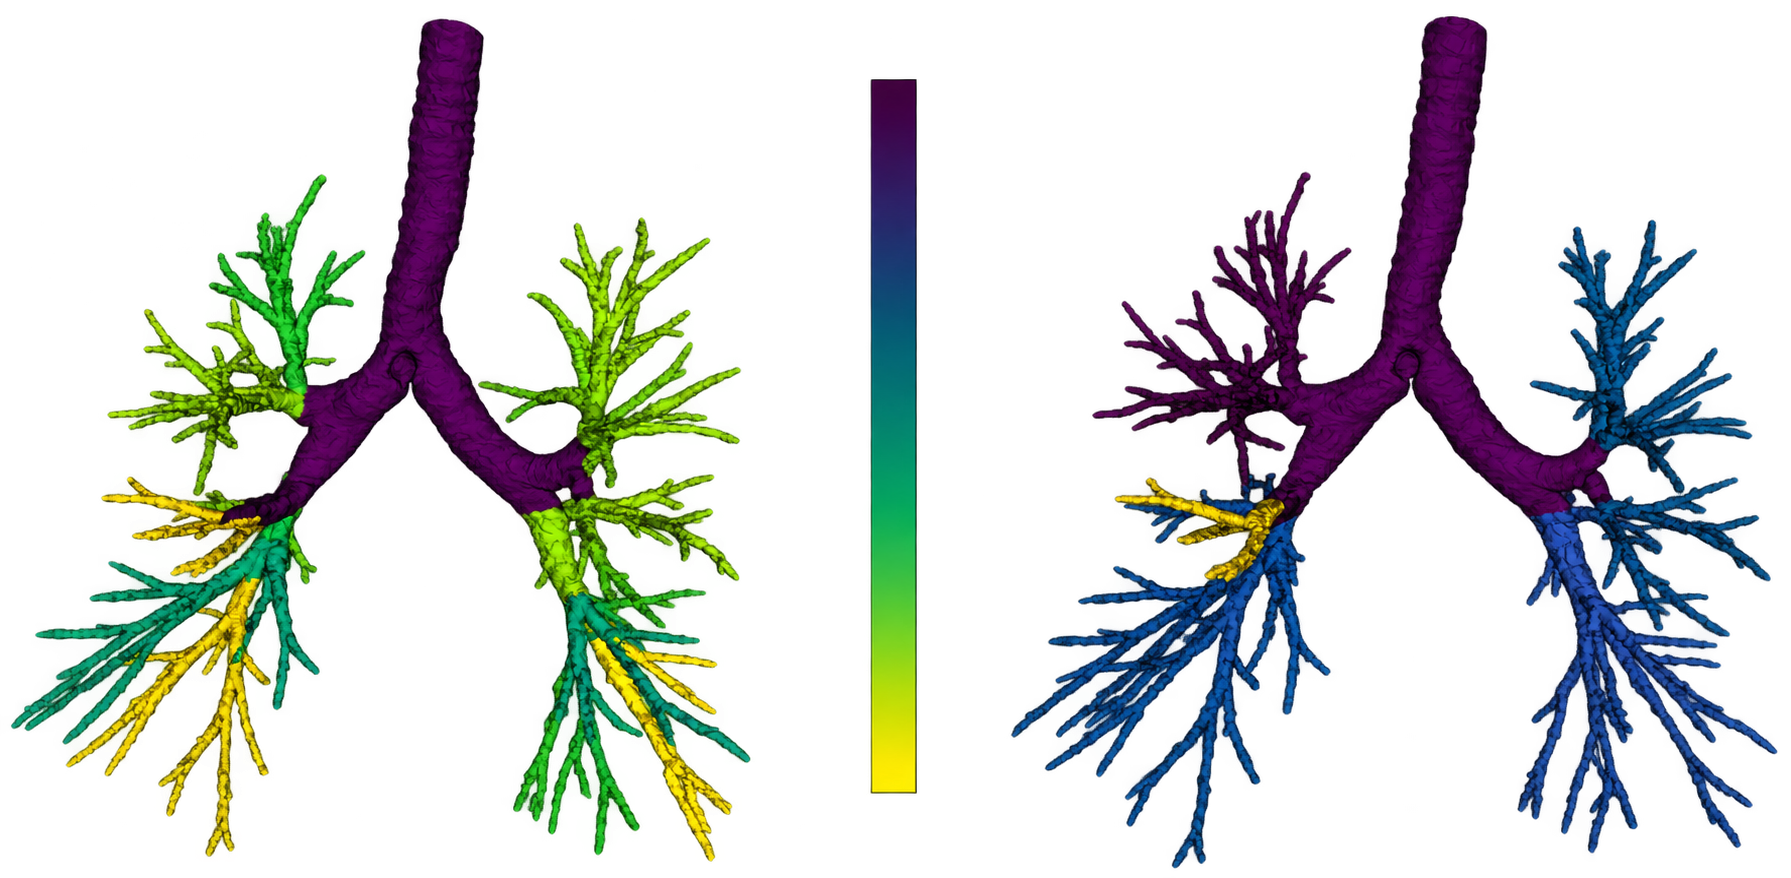
\includegraphics[width=\textwidth]{figures/morph_signatures_ours.png}  % uncomment with your file
  \caption{Examples of airway trees visualized according to the Ectasia descriptor of
            AirwaySignature \cite{zhang2025airmorph}. The left panel shows Ectasia values computed
            at the segmental level, with each color corresponding to an individual segmental
            bronchial class. The right panel shows the same descriptor computed at the lobar level,
            after grouping the corresponding segmental branches within each lobe. The common color
            scale indicates the magnitude of ectasia, with warmer colors corresponding to greater
            airway dilation relative to the mean branch radius.}
  \label{fig:morph_ours}                 % referenced as Figure~\ref{fig:morph_ours}
\end{figure}
